\documentclass{article}

% Language setting
% Replace `english' with e.g. `spanish' to change the document language
\usepackage[english]{babel}

% Set page size and margins
% Replace `letterpaper' with`a4paper' for UK/EU standard size
\usepackage[a4paper,top=2cm,bottom=2cm,left=2cm,right=2cm,marginparwidth=1.75cm]{geometry}

% Useful packages
\usepackage{amsmath}
\usepackage{graphicx}
\usepackage[backend=biber,
style=chem-angew,
sorting=none
]{biblatex}
\addbibresource{sample.bib}
\usepackage[colorlinks=true, allcolors=blue]{hyperref}

\title{Data Analysis in \textit{"Trophic allometry in a predator that carries corpses of its prey"}}
\author{Nicole Riatto Victor}
\date{}

\begin{document}
\maketitle

This work was done based in the data present in Victor \& Costa-Pereira (2022) \cite{victor2022trophic}.

\section{Introduction}

The allometric scaling approach is a powerful tool to predict ecological interactions \cite{garlaschelli2003universal}. Trophic links are especially determined by biomechanical mechanisms and the relative body size of predators and their prey (i.e., trophic allometry). For instance, a predator's body size is often related to its metabolic rate, strength, and speed, which are traits that determine its efficiency in searching, subjugating, and consuming prey \cite{wootton2021towards}. In turn, a prey's body size is associated with its energy content and diverse antipredator strategies \cite{portalier2019mechanics}. Therefore, ecological theory predicts that there should be an optimal predator–prey size ratio (PPSR) that maximizes the predator's energy gain \cite{griffiths1980foraging}. However, many examples in nature show that predators choose their prey not only seeking to optimize energy intake \cite{paine1966food}.
\\

The nymphs of ant-snatching assassin bugs of genera \textit{Acanthaspis} Amyot and Serville 1843 and \textit{Inara} Stål 1859 (Hemiptera: Reduviidae) use their prey not only to obtain energy and nutrients but also for camouflage \cite{jackson2007bugs,odhiambo1958some}. These small voracious predators cover themselves with the remains of their prey, creating a ‘backpack’ (or a ‘mask’) made of ant carcasses (Figure \ref{figure_bugs}). This strategy of covering the body with foreign material is known as masking (or decorating) \cite{ruxton2015evolutionary}. This backpack of corpses increases assassin bug's survival chances against visually oriented predators by avoiding their recognition as prey \cite{brandt2002bugs,jackson2007bugs}. This peculiar behavior of ant-snatching assassin bugs makes them an interesting model to understand the allometry of trophic interactions because they (i) carry a ‘history’ of several past foraging events on their backpack (which allows us to quantify prey traits) and (ii) might capture their prey not only taking into account the maximization of energy gain, but also the increase in camouflage efficiency.
\\

\begin{figure}
    \centering
    \includegraphics[width = 0.5\textwidth]{Figure_1.jpg}
    \caption{Two individuals of ant-snatching assassin bugs carrying a backpack made of carcasses of their favorite prey (ants). This photograph was not used to collect data for this study because assassin bugs are not in a lateral view. Photographer: Melvyn Yeo (\url{https://flic.kr/ps/2iz6em}).}
    \label{figure_bugs}
\end{figure}

Here, I used photographs of \textit{Acanthaspis} spp. and \textit{Inara} spp. nymphs to study the still poorly explored trophic ecology of ant-snatching assassin bugs. First, I used photographs of these predators to describe (i) the relative size of predators and prey (predator–prey size ratios, PPSR) and (ii) the number of prey carcasses carried by each predator. Then, I tested whether there is a trade-off between PPSR and the number of ant carcasses present in an individual's backpack. I predict that the larger the size of the prey relative to the predator (i.e., lower PPSR) the smaller the number of ants present in the assassin bug's backpack. I expect this pattern because small assassin bugs should not be able to capture and carry relatively large ants, while large predators would have increased costs associated with searching and capturing numerous small prey.

\section{Methods}

I searched for photographs of \textit{Acanthaspis} and \textit{Inara} individuals in online public image repositories (\textit{Deviant Art, Flickr, iNaturalist};
search term: “assassin bug”) and selected those that showed the assassin bugs in a side view. This criteria was important to allow for accurate measures of my variables of interest. The morphological distinction between the two genera I studied can only be made in the adult stage,
which was impossible since I was using photographs. In each selected photograph, I quantified my two operational variables: PPSR and the number of prey. 

\subsection{Quantifying PPSR}

As PPSR is dimensionless, I measured the size of the predator and the prey in pixels using the ImageJ software \cite{abramoff2004image} since in the photographs there was no scale to know their real size. The predator size was measured by its body length (from the tip of the rostrum to the tip of the abdomen). Even though it was not possible to identify the species of ants, carcasses present on the backpack of each assassin bug have very similar sizes and shapes. Therefore, I assumed that all ants on a given backpack have the same body size. Considering how the ants are aggregated, it is not feasible to accurately measure their body length in the photographs. Thus, I used the head length (from the mid-point of the anterior clypeal margin to the mid-point of the posterior margin) as a proxy for prey size because this dimension is isometric with body length \cite{tschinkel2013morphometry}. In all selected photographs, at least one head was in a front view. The measures of the ant head length and the bug body length of each photograph are inside 'data/raw/data-ppsr.csv'. 

\subsection{Quantifying the number of ants in each backpack}

I also used a mathematical approximation to estimate the number of ants present in the predator's backpack as it was not possible to count them precisely from the photographs. First, I calculated the volume of a single ant based on Tschinkel (2013), which indicates that the gaster volume of \textit{Solenopsis} represents approximately 57\% of its total body volume. I used this proportion for all ants because this fine allometric characterization has rarely been estimated for other genera. Then, assuming that the ant's gaster is a spheroid \cite{tschinkel2013morphometry}, I also measured its length (GL) and width (GW) with ImageJ software \cite{abramoff2004image}. These two metrics are inside 'data/raw/data-ant-gaster.csv'. I used Equation 1 to quantify the gaster volume (a = GL and b = GW). Second, given the way carcasses of ants are arranged (Figure 1), I also considered the predator's backpack as a spheroid. I measured its length (BL) and height (BH) in ImageJ software \cite{abramoff2004image} and the values are in 'data/raw/data-backpack.csv'. To quantify its volume, I also used the same Equation 1 (a = BL and b = BH). After calculating the two volumes (of the backpack and of an ant), I used the maximally random jammed (MRJ) parameter of $\sigma$ = 0.637 \cite{donev2004improving} to estimate the percentage of the backpack volume occupied by ants. This empirical parameter represents the relative volume of amorphous objects packed randomly \cite{donev2004improving}. Then, I divided the resulting occupied volume by the volume of an individual ant to estimate the total number of ants. All the mathematical operations were done in R \cite{rstudio} and the code can be found in more details in ´scripts/01\_manipulation\_data.R´ directory.

\begin{equation}
    V = \frac{4}{3}\pi(\frac{a}{2})(\frac{b}{2})^{2}
\end{equation}

\subsection{Descriptive and statistical analysis}

I also did a descriptive analysis of the data obtained. In R, I created two raincloud plots with the distribution of the PPSR and the number of ants. The code is available in `scripts/02\_plots.R`. Furthermore, to test if there is a positive relation between the number of carried ant carcasses and the relative size of predators and their prey, I fitted a Generalized Linear Model with Poisson distribution. I selected this type of GLM because the number of ants is a discrete variable and it represents a count. Also, the relationship seems to be logarithmic. PPSR was included as the predictor variable and the number of ants in the backpack as the response variable. The code is available in `scripts/03\_models.R`.

\section{Results}

The number of carcasses carried by ant-snatching
assassin bugs varied widely, while one individual carried only three ants, another carried approximately 102 ants (average = 48.69, SD = 28.526). The relative size of predator nymphs and their prey also showed substantial variation. While some predators were about three times longer than the head of their prey, other predators were 10 times longer (average = 7.237,
SD = 1.723). Predators that consumed relatively large ants (i.e., low PPSR) carried fewer prey in their backpack ($\beta_1 = 0.25 \pm 0.01$,
$p_r(>|z|) < 0.0001$) (Figure \ref{figure_plots}). 
\\

\begin{figure}
    \centering
    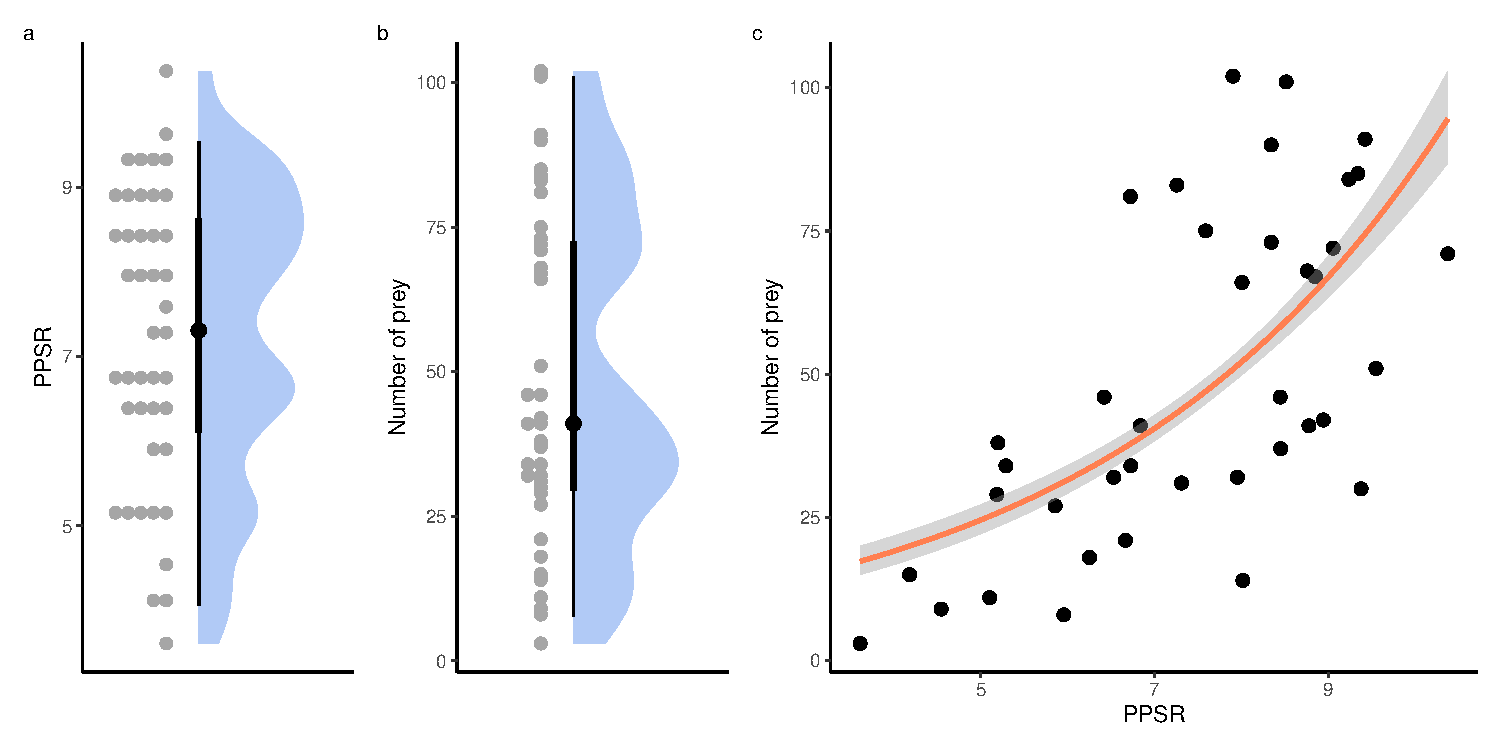
\includegraphics[width = \textwidth]{figure_plots.pdf}
    \caption{Raincloud plots showing density distributions, data points, and summary statistics (median and interquartile range) for (a) the
number of prey carcasses carried and (b) predator–prey
size ratio (PPSR) in 43 ant-snatching
assassin bugs nymphs. (c) Relationship between
the number of ants in the backpack and the relative size of the predator and its prey (i.e., large PPSR values correspond to predators that
carry relatively small prey)}
    \label{figure_plots}
\end{figure}

My results corroborate with the enduring principle that body size is a key trait shaping trophic interactions \cite{petchey2008size}. Classical studies on trophic allometry suggested that there should be an optimal and universal theoretical value of PPSR, at which the energy return is maximized \cite{emerson1994allometric, west1997general}. However, recent studies question this hypothesis, as PPSRs in natural systems are flexible and context-dependent. Indeed, I observed a large variation in PPSR across predators. This way, other traits, such as defensive traits and cuticle thickness and hardness, may also play a role in these consumption patterns.
\\

I also found that the larger the relative size of the ant, the smaller the number of prey in the backpack. The antipredator behavior of carrying prey carcasses incurs in additional energetic costs for assassin bugs \cite{ruxton2015evolutionary}. Therefore, biomechanical limitations should determine not only PPSRs \textit{per se} but also the number of ants carried in the backpack \cite{charnov1976optimal}. For instance, even if highly effective for camouflage purposes, a pack consisting of numerous large prey (i.e., low PPSR) would be highly costly because bigger ants take more energy to carry than smaller ones. Moreover, the volume of the backpack may also be a relevant limiting factor, as there is a finite availability of space (determined by the size of the predator's back) that can be occupied by ant carcasses. Thus, my results support the hypothesis that there is a trade-off between PPSR and the number of prey used to avoid predators via masking, which has implications not only for the foraging of assassin bugs but also for their defense from predators.

\printbibliography[title={References}]

\end{document}